\documentclass[a4paper]{article}
\usepackage{hyperref}
\usepackage{graphicx}
\usepackage{amsmath,amsfonts,amsmath,amsthm,amssymb}
\usepackage{caption}
\usepackage{multirow}
\usepackage{physics}
\usepackage{tikz}
\usepackage{cleveref}
\usepackage{pgfplots}
\usepackage{pgfplotstable}
\usepackage{siunitx}
\usepackage{wrapfig}
\usepackage{graphicx}
\usepackage{subfiles}
\usepackage{bm}
\usepackage{xcolor}
\usepackage[french]{babel}
\usepackage{titlesec}
\usepackage{lmodern}
\usepackage{braket}
\usepackage{geometry}
 \geometry{
 a4paper,
 total={170mm,257mm},
 left=20mm,
 top=20mm,
 }

\numberwithin{equation}{part}

\pgfplotsset{width=10cm,compat=1.16}

\newcommand{\ti}{\times}
\newcommand{\h}{\hbar}


\titleformat{\paragraph}
{\normalfont\normalsize\bfseries}{\theparagraph}{1em}{}
\titlespacing*{\paragraph}
{0pt}{3.25ex plus 1ex minus .2ex}{1.5ex plus .2ex}

\title{\textbf{PHYS-F203 - Introduction à la Mécanique Quantique} \\ Basé sur les notes de Prof. Serge MASSAR}
\author{MOEIL Juian}
\date{\textbf{Année académique 2020-2021}}

\newtheorem{theorem}{Théorème}[section]
	\newtheorem{definition}{Définition}[section]
\newtheorem{lemma}{Lemme}[section]
\newtheorem{Property}{Proposition}[section]
\newtheorem{corollary}{Corollaire}[section]
\newtheorem{remark}{Remarque}[section]
\newtheorem*{preuve}{Preuve}
\newtheorem{reminder}{Rappel théorique}[section]
\newtheorem{exemple}{Exemple}[section]

\renewcommand\qedsymbol{$\blacksquare$}

\begin{document}

\maketitle
\begin{center}
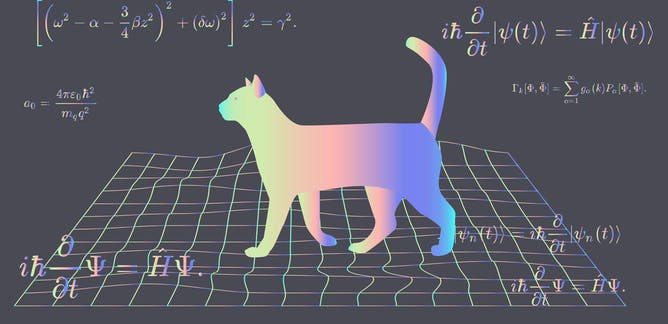
\includegraphics[scale=0.65]{Images/cat.jpg}
\end{center}
\begin{center}

\includegraphics[scale=0.20]{Images/sciences.png}
\end{center}
\begin{center}

\includegraphics[scale=0.45]{Images/ULB.jpg}
\end{center}

\newpage
\textbf{Avertissement.} Dans le cadre de ce document, nous définissons le symbole $\doteq$ comme signifiant "par définition". Les vecteurs seront indiqués en gras : $\vec{x} = \bm{x}$.
\tableofcontents

\newpage
\subfile{Chapitre 1/chapitre1.tex}
\newpage
\subfile{Chapitre 2/chapitre2.tex}
\newpage
\subfile{Chapitre 3/chapitre3.tex}
\newpage
\subfile{Chapitre 4/chapitre4.tex}
\newpage
\subfile{Chapitre 5/chapitre5.tex}

\newpage
\subfile{Annexe/annexe.tex}

\end{document}